\documentclass[11pt]{article}
\usepackage{amsmath,array}
\usepackage{amsfonts}
\usepackage{amssymb}
\usepackage{amsthm}
\usepackage{graphicx,subcaption}
\usepackage{todonotes} %[disable]
\usepackage{cleveref}
\usepackage{tikz}
\usepackage{placeins} %FloatBarrier
\usetikzlibrary{arrows,shapes,calc}
\tikzset{line/.style = {draw, -latex'}}
\newcommand{\abs}[1]{\left|{#1}\right|}
\newcommand{\pde}[2]{{\frac{\partial {#1}}{\partial {#2}}}}
\newcommand{\pdde}[2]{\frac{\partial^2 {#1}}{\partial {#2}^2}}
\newcommand{\de}[2]{\frac{\mathrm{d} #1}{\mathrm{d} #2}}
\newcommand{\dde}[2]{\frac{\mathrm{d}^2 {#1}}{\mathrm{d} {#2}^2}}
\newcommand{\intdef}[4]{\int\limits_{#1}^{#2} #3\, \mathrm{d}{#4}}
\crefname{appendix}{Appendix}{appendices}
\crefname{section}{Section}{sections}
\crefname{table}{Table}{tables}
\Crefname{table}{Table}{Tables}
\crefname{algorithm}{Algorithm}{algorithms}
\Crefname{algorithm}{Algorithm}{Algorithms}
\crefname{equation}{Eq.}{eqs.}
\Crefname{equation}{Equation}{Equations}
\crefname{figure}{Fig.}{figs.}
\Crefname{figure}{Figure}{Figures}
\crefname{subfigure}{Fig.}{figs.}
\Crefname{subfigure}{Figure}{figures}
\captionsetup[subfigure]{labelformat=simple}
\renewcommand{\thesubfigure}{(\alph{subfigure})}
\renewcommand{\vec}[1]{\boldsymbol{#1}}
%opening
\title{Correctly inferring causal connectivity using optogenetics}
\author{Mikkel Elle Lepper\o{}d, Konrad Paul Kording}

\begin{document}

\maketitle

\begin{abstract}
\noindent Neurons interact through spikes and a central objective of neuroscience is measuring the way how neurons causally affect one another. To probe such interactions, scientists often use optogenetics which typically leads to stimulation effects on multiple cells. This then produces a so-called confounding problem - we cannot know which of the stimulated neurons affected the activity of a given target neuron. Here we show how the resulting biases are large and how causal inference techniques, in particular instrumental variables, from econometrics can ameliorate this problem. Our approach utilizes the fact that neurons have absolute refractory times where the stimulation has no influence, and the missing stimulation acts like an effectively random variable which can then be used to disentangle causality. If we can not apply truly random stimulation to a network of neurons then causal inference techniques are needed to identify mechanisms.
\end{abstract}

\section{Introduction}
% neuroscience experiments are observational which implicates a certain set of statistical tools
% spike timing cannot give a causal estimate of connectivity, thus we need to perturbe the system
%a quest for causality and optogenetics is a main tool

%set up the drive to causality
We want mechanism. Seriously. Neuroscience is to a large part experimentally driven.

%we generally use observational studies
We use observational studies. But causality is typically wrong. <nutshell version of the mehler paper>

%set up confounding
 The experiments are extremely hard to control, even with the most accurate measurements of environmental variables and minimal genetic variance. Actually, given the vast amount of neurons and their connections in primitive mammals experiments are to be considered an observational sort. In a quest for experimental control we are now able to measure from thousands of neurons at the same time with micro-second precision by electrophysiology or with high spatial accuracy by two photon imaging. However, the large amount of unmeasured activity makes estimates of functional connectivity confounded. By confounded we mean that correlations between neuron pairs are largely influenced by the background activity. One example of this confounding is when two neurons $ A,B $ are driven by a common input $ D $, while one wants to estimate connectivity between $ A $ and $ C $. However only $ B $ and C is connected such that B and C are strongly correlated, then since $ B $ and $ C $ is correlated then $ A $ and $ C $ is correlated and a regression $ C = \beta A $ will give an erroneous $ \beta > 0 $ due to the the $ A,B $ correlation given by their common input $ D $. In this case we say the regressor $ A $ is endogenous and the regression coefficient $ \beta $ estimates the magnitude of association rather than the magnitude of causation. To estimate causal relationships between neurons, stimulation is appropriate, and if able to stimulate single neurons the ability to estimate causal relationships by regression is within grasp. However, this is experimental challenging and yield very low cell count. Therefore an optogenetic approach is more than often preferable.

%optogenetics is totally nonlocal
Within the bounds of reachable tissue for photons emitted by a light source the decay of light intensity decays proportional to $ 1/r^2 $. Furthermore if the distribution of neurons is homogeneous the probability of affecting a neuron increases in distance by $ r^2 $. This essentially makes the distribution of affected neurons flat. When performing simultaneously recording with optogenetic stimulation we again get a confounding problem when estimating the functional relationships between neuron pairs. In this case the confounding is when several neurons see the same stimulus and thus become highly correlated during stimulation yielding statistically indistinguishable functional relationships, this case is similar to the above example where $ D $ now is the optogenetic stimulation. Flat distribution of V.

%causal inference is a thing, if not done well you say stupid things
The problem of endogenous regressors is common in microeconomics and in the social sciences\todo{cite}, where observed outcomes can be driven by a large number of unknown factors. It is thus largely recognized that special care has to be taken when attempting to infer causal relationships between a putative actor and an outcome. 

%example
Let's say that you want to estimate the return $ \beta $ from education $ x $ to yearly income $ y $ with the regression $ y = \beta x + u $, where $ u $ is the factors other than schooling that contributes to yearly income. One of the factors in $ u $ is a persons ability, however this may also affect schooling and thus the regressor is correlated with the error term and a regression estimate will not estimate the magnitude of causation from schooling. In this case one may use the proximity to a college or university as an instrumental variable (IV) $ z $\todo{cite card 1995, found in cameron}. There are two criterion that must be fulfilled when choosing an instrumental variable, the instrument must be (1) uncorrelated with the error term, and (2) correlated with the regressor $ x $. Then one may for instance estimate $ \beta $ by a two stage ordinary least squares (OLS) where the first stage is an OLS of the regressor and the instrument which is further used in the second stage with the dependent variable $ y $\todo{cite TSOLS}. summary sentence.

%worry is this really correct? Yes, its provable. 
worry is this really correct? Yes, its . IVs are (under the right assumptions) actually correct.

%here we
The IV technique can also be employed if one seeks to estimate the causal connectivity between neuron pairs. In this study we begin by showing how a simple network of three leaky integrate and fire (LIF) neurons can be heavily confounded under the right circumstances when simulating optogenetic targeting as direct current pulses. We then show that using the refractory period as an instrumental variable we are able to produce good estimates of causal connectivity. Furthermore we show that the method works in a large (N=1250) network of LIF neurons. With this data at hand we compare the IV method with a logistic regression.

\section{Results}
\begin{figure}
\makeatletter
\renewcommand\p@subfigure{}
\makeatother
\begin{subfigure}{\textwidth} 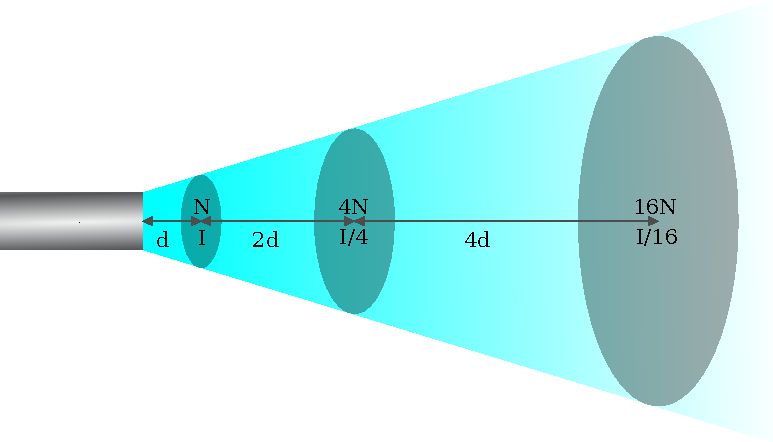
\includegraphics[scale=1]{light-decay}
\caption{} \label{fig:concept:1}
\end{subfigure}

\medskip
\begin{subfigure}{\textwidth} 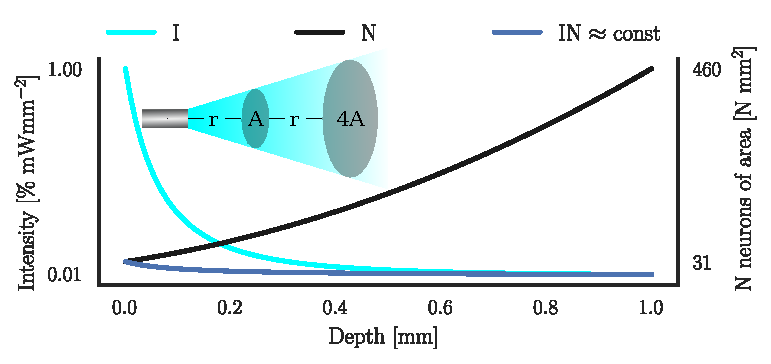
\includegraphics[scale=1]{opto-powerlaw}
\caption{} \label{fig:concept:2}
\end{subfigure}
\caption{Sketch of the problem at hand \label{fig:concept}}
\end{figure}
\todo[inline]{perturbation should spread by 1/r2 and all perturbed connections should be tested, here logit will fail.}
\todo[inline]{figure showing stimulating of network}
\todo[inline]{figure comparing methods with real weights}
\todo[inline]{figure showing power (true false vs n stimulations)}
\todo[inline]{data showing false positive/negative comparing stimulation patterns, comparing stimulation durations}
\todo[inline]{data showing synchrounous regular does not work (can be put together with regular stim. pattern)}
\todo[inline]{Should we show that ccg or gml give lots of false positives? without considering stimulation?}
\todo[inline]{I think I would choose a couple of examples that emulate what an experimentalist would do
(a) periodic slow (bad power not enough data)
(b) periodic fast (good power but confounded)
(c) random fast (good everything)
But I would then also redo all of them with a "weak network" model where therefore the assumptions are pretty well matched an also a "strong network" model where neurons have massive influence on one another (maybe oscillate or something) and hence the weakness assumption that is behind the IV justification breaks down }
Consider three neurons (A,B,C) where A and B receives optogenetic stimulation and only B is connected to C \cref{fig:intro}\labelcref{fig:intro:1}. The stimulation induces a strong correlation between A and B \cref{fig:intro}\labelcref{fig:intro:1,fig:intro:2,fig:intro:3,fig:intro:4}, and thus the monosynaptic connection between B and C is thus spuriously inherited between A and C confounding the system by rendering the cross correlation histograms (CCHs) between BC and AC statistically indistinguishable as seen in \cref{fig:intro}\labelcref{fig:intro:5,fig:intro:6} respectively.
\begin{figure} 
\makeatletter
\renewcommand\p@subfigure{}
\makeatother
\begin{subfigure}{0.485\textwidth} 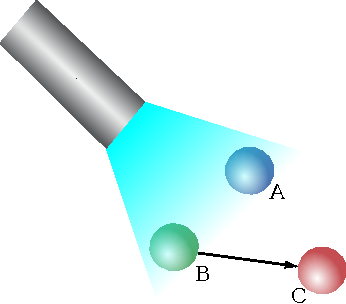
\includegraphics[scale=1.3]{simple}
\caption{} \label{fig:intro:1}
\end{subfigure}\hfill
\begin{subfigure}{0.485\textwidth} 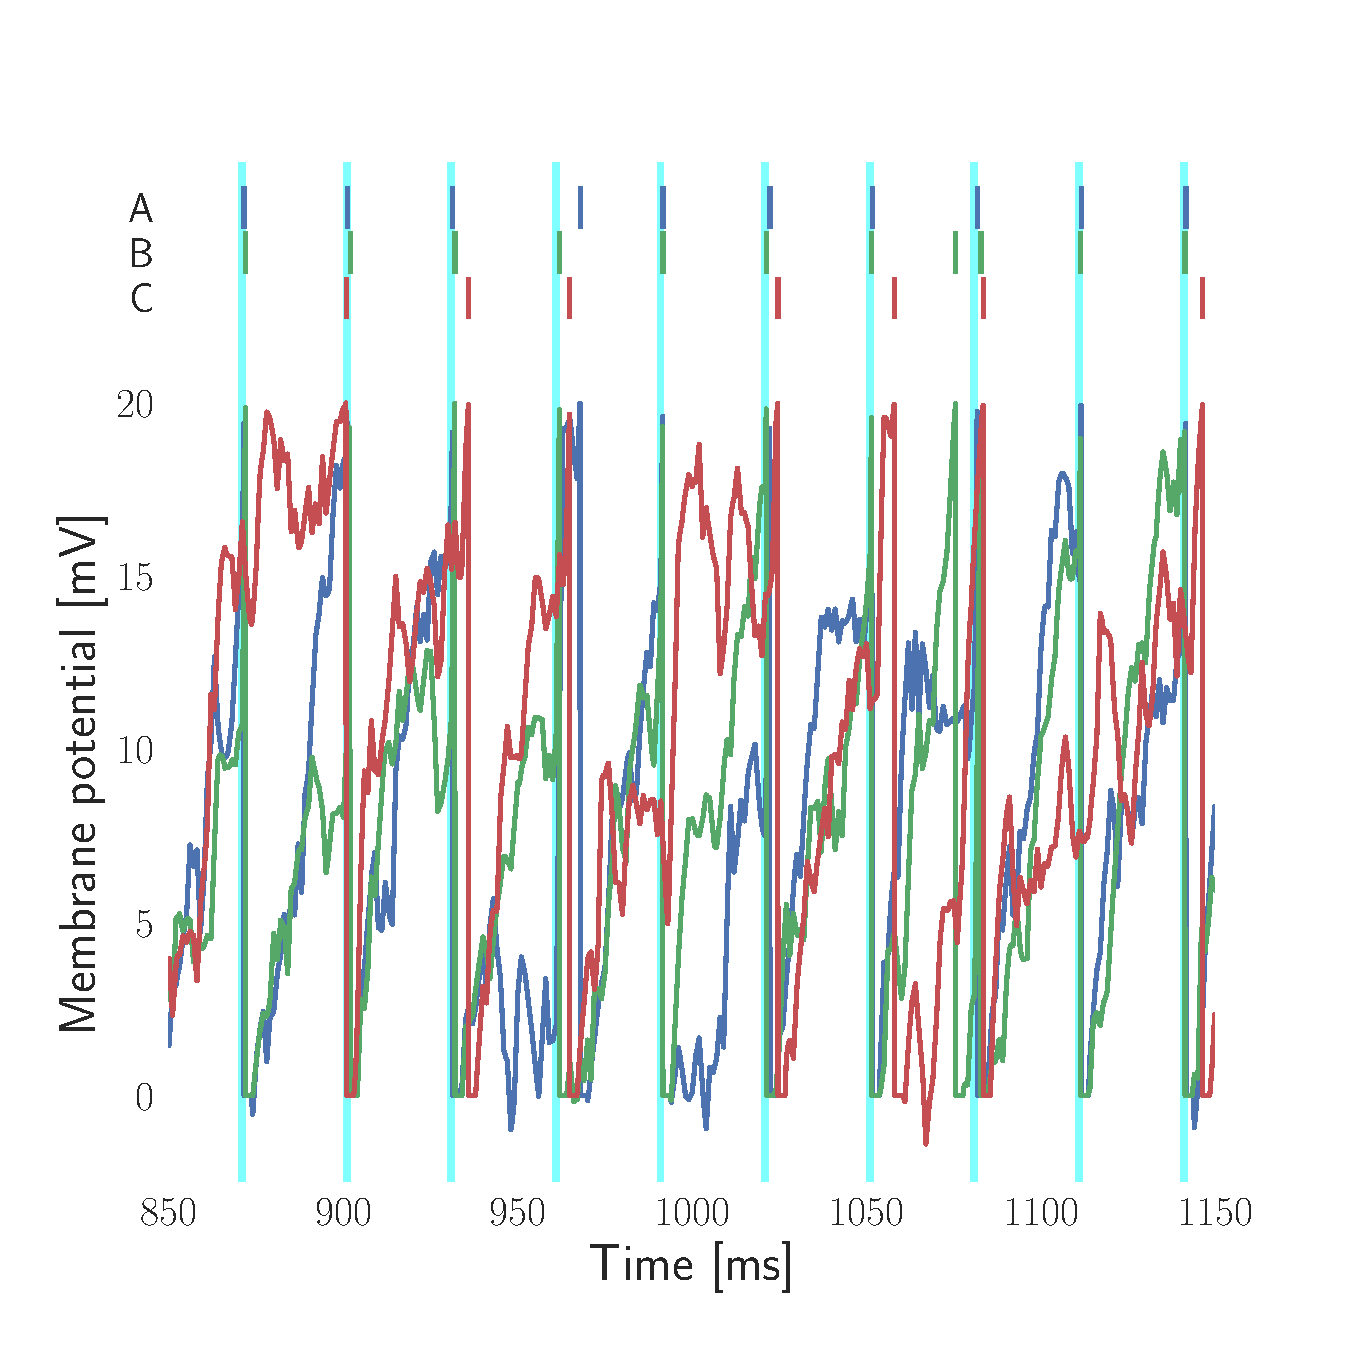
\includegraphics[scale=.25]{traces}
\caption{} \label{fig:intro:2}
\end{subfigure}

\medskip
\begin{subfigure}{0.485\textwidth} 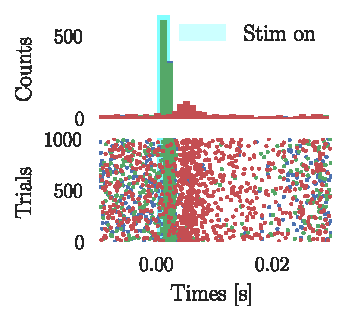
\includegraphics[scale=.25]{raster}
\caption{} \label{fig:intro:3}
\end{subfigure}\hfill
\begin{subfigure}{0.485\textwidth} 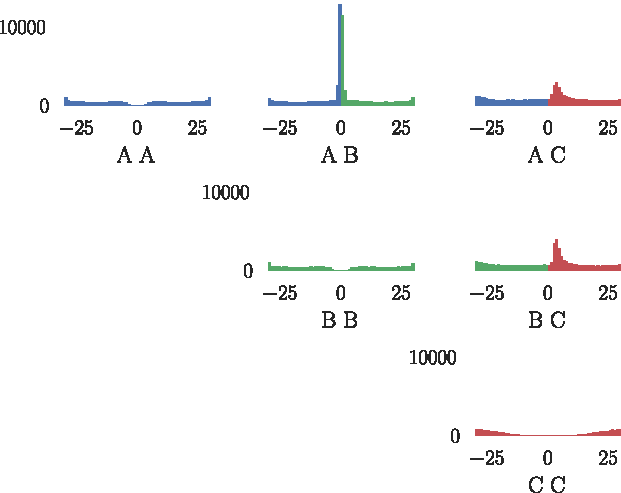
\includegraphics[scale=.25]{xcorr}
\caption{} \label{fig:intro:4}
\end{subfigure}
\caption{Sketch of a simple network containing three neurons depicted in red stimulated with blue laser light trough optogenetic activation. Invoked spikes due to stimulation is depicted in (b) upper panel with corresponding voltage traces in the lower panel. The neurons A and B are stimulated multiple trials and the  histogram of all trials are shown in (c) upper panel with the corresponding raster plot for each trial in the lower panel. Horizontal and vertical axes in correlograms represents respectively time lag in ms and counts of coincident spikes in bins of 1 ms for \labelcref{fig:intro:4} \label{fig:intro}}
\end{figure}

\begin{figure}
\begin{subfigure}{0.485\textwidth} 
\includegraphics[scale=.25]{xcorr_highres_BC}
\caption{} \label{fig:cchvswald:1}
\end{subfigure}\hfill
\begin{subfigure}{0.485\textwidth} 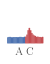
\includegraphics[scale=.25]{xcorr_highres_AC}
\caption{} \label{fig:cchvswald:2}
\end{subfigure}

\medskip
\begin{subfigure}{0.485\textwidth} 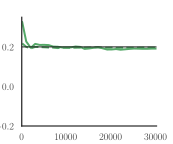
\includegraphics[scale=.25]{wald_BC}
\caption{} \label{fig:cchvswald:3}
\end{subfigure}\hfill
\begin{subfigure}{0.485\textwidth} 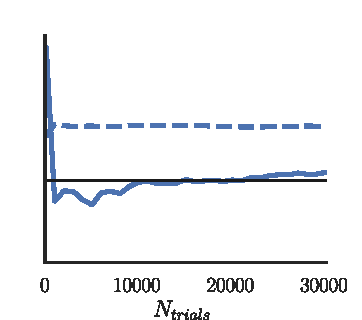
\includegraphics[scale=.25]{wald_AC}
\caption{} \label{fig:cchvswald:4}
\end{subfigure}
\caption{Cross correlograms for all neurons are depicted in (d) and the high resolution zoom of BC and AC are visualized in (e) and (f) respectively. Horizontal and vertical axes in correlograms represents respectively time lag in ms and counts of coincident spikes in bins of 0.1 ms for \labelcref{fig:cchvswald:1,fig:cchvswald:2}. \label{fig:cchvswald}}
\end{figure}

\begin{figure}
\makeatletter
\renewcommand\p@subfigure{}
\makeatother
\begin{subfigure}{0.485\textwidth} 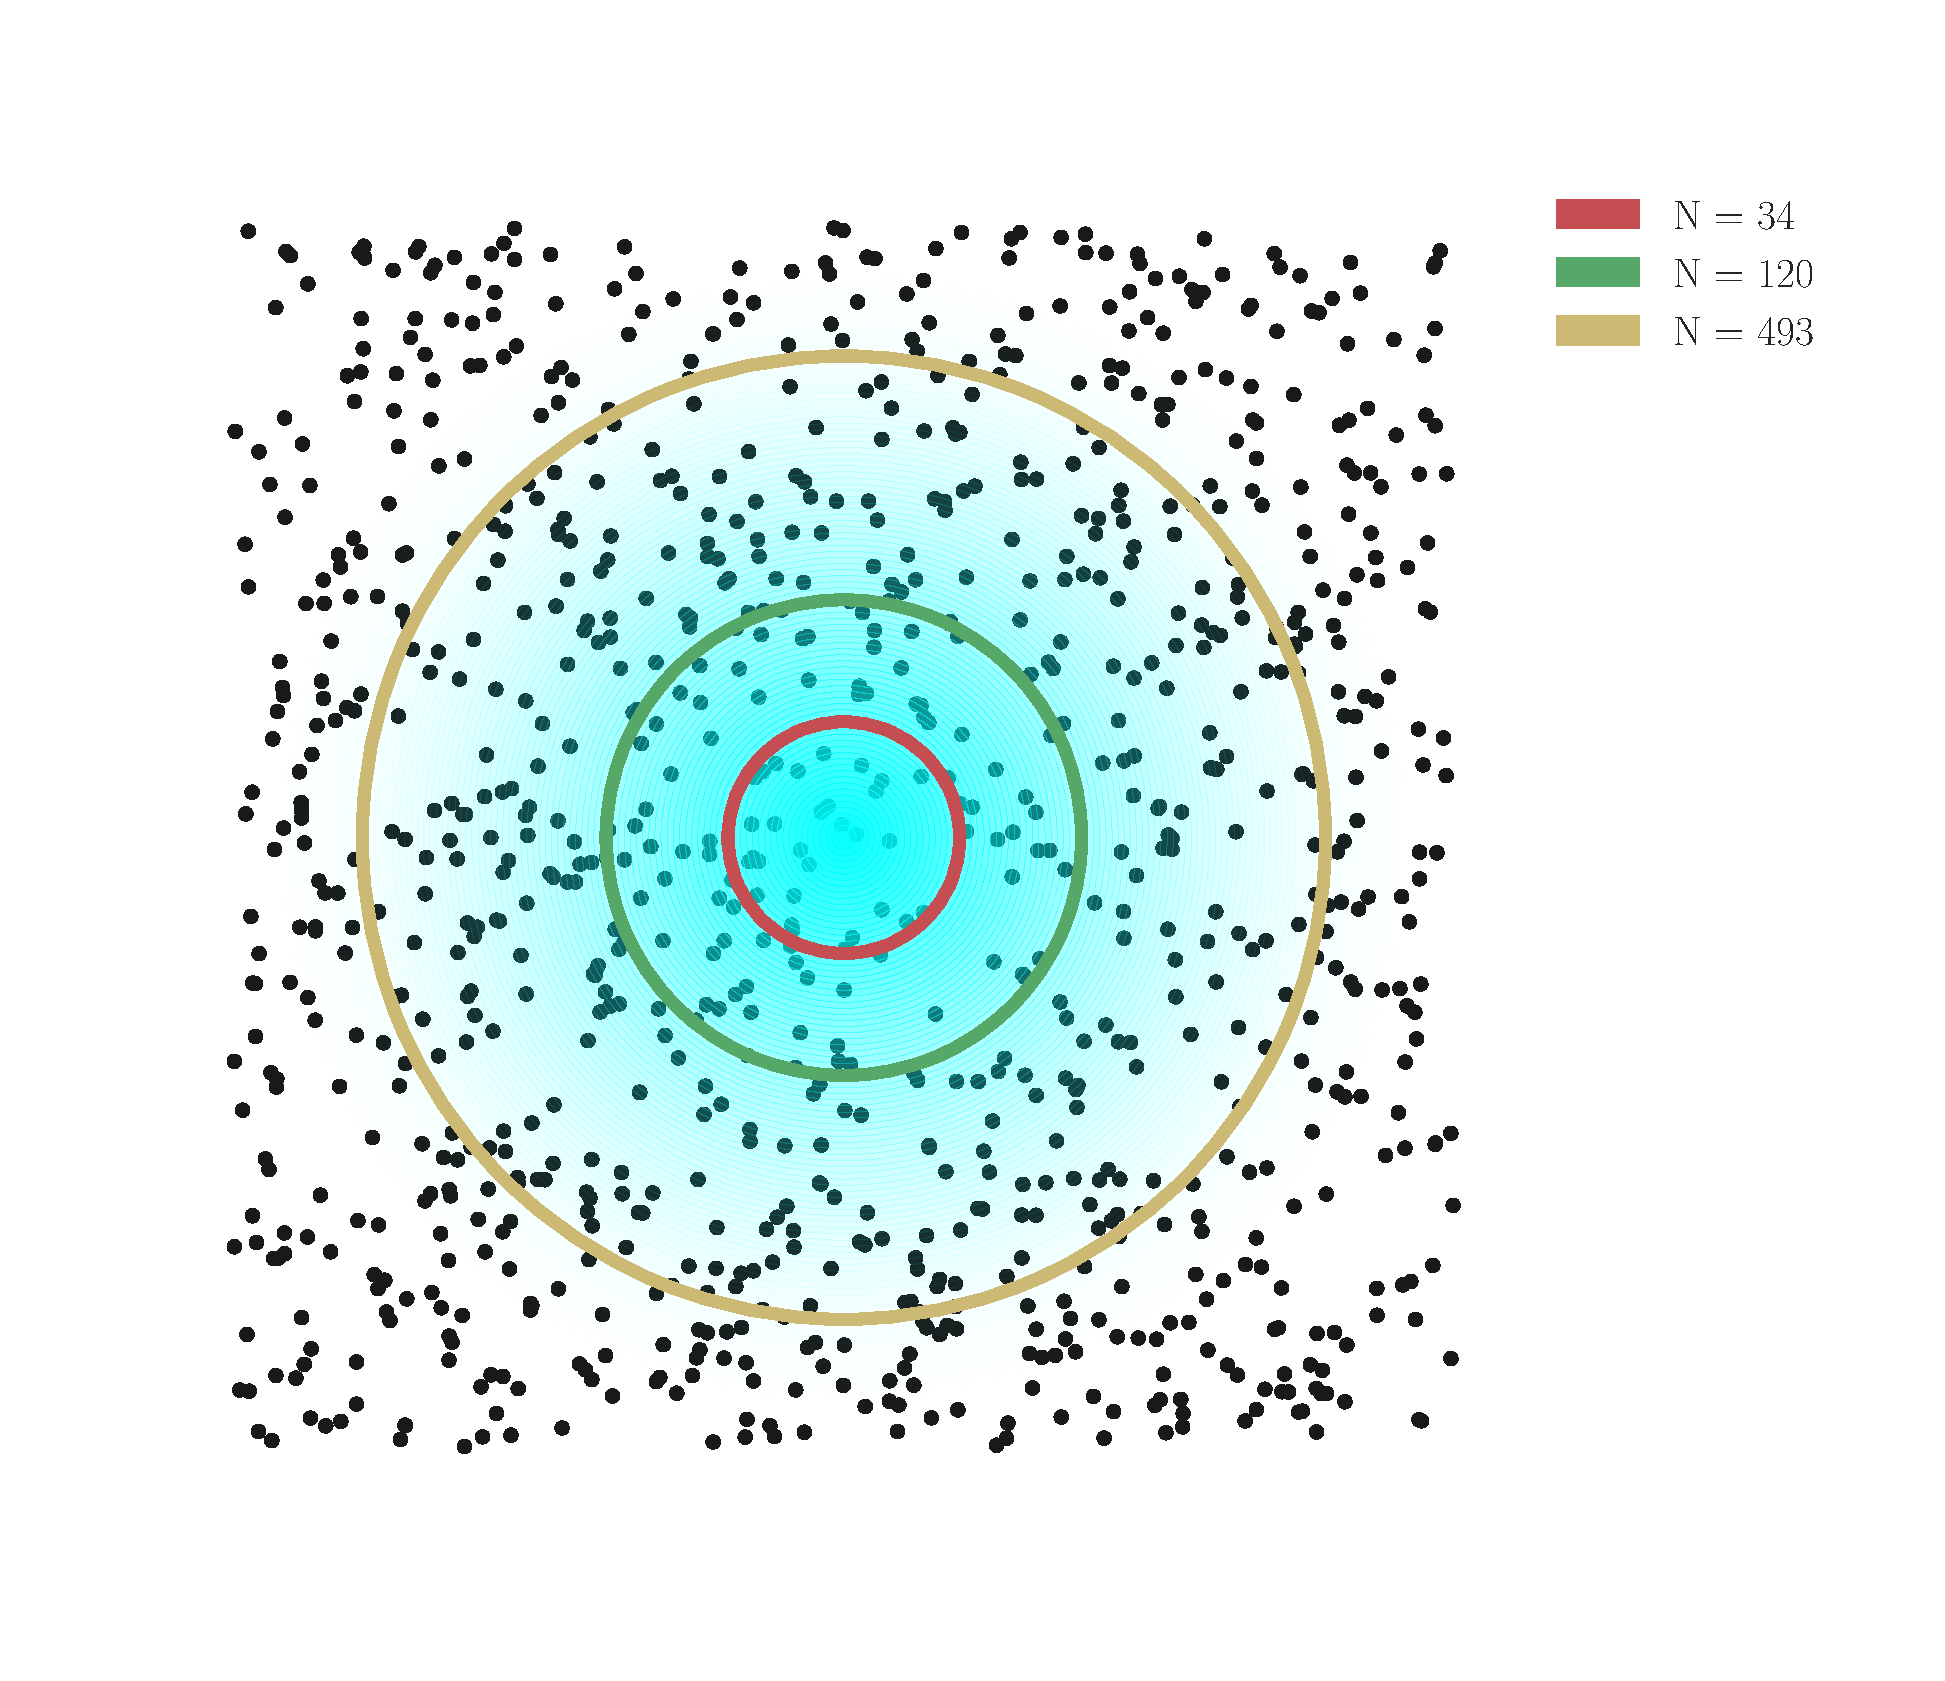
\includegraphics[scale=.2]{network_stim}
\caption{} \label{fig:network-power:1}
\end{subfigure}\hfill
\begin{subfigure}{0.485\textwidth}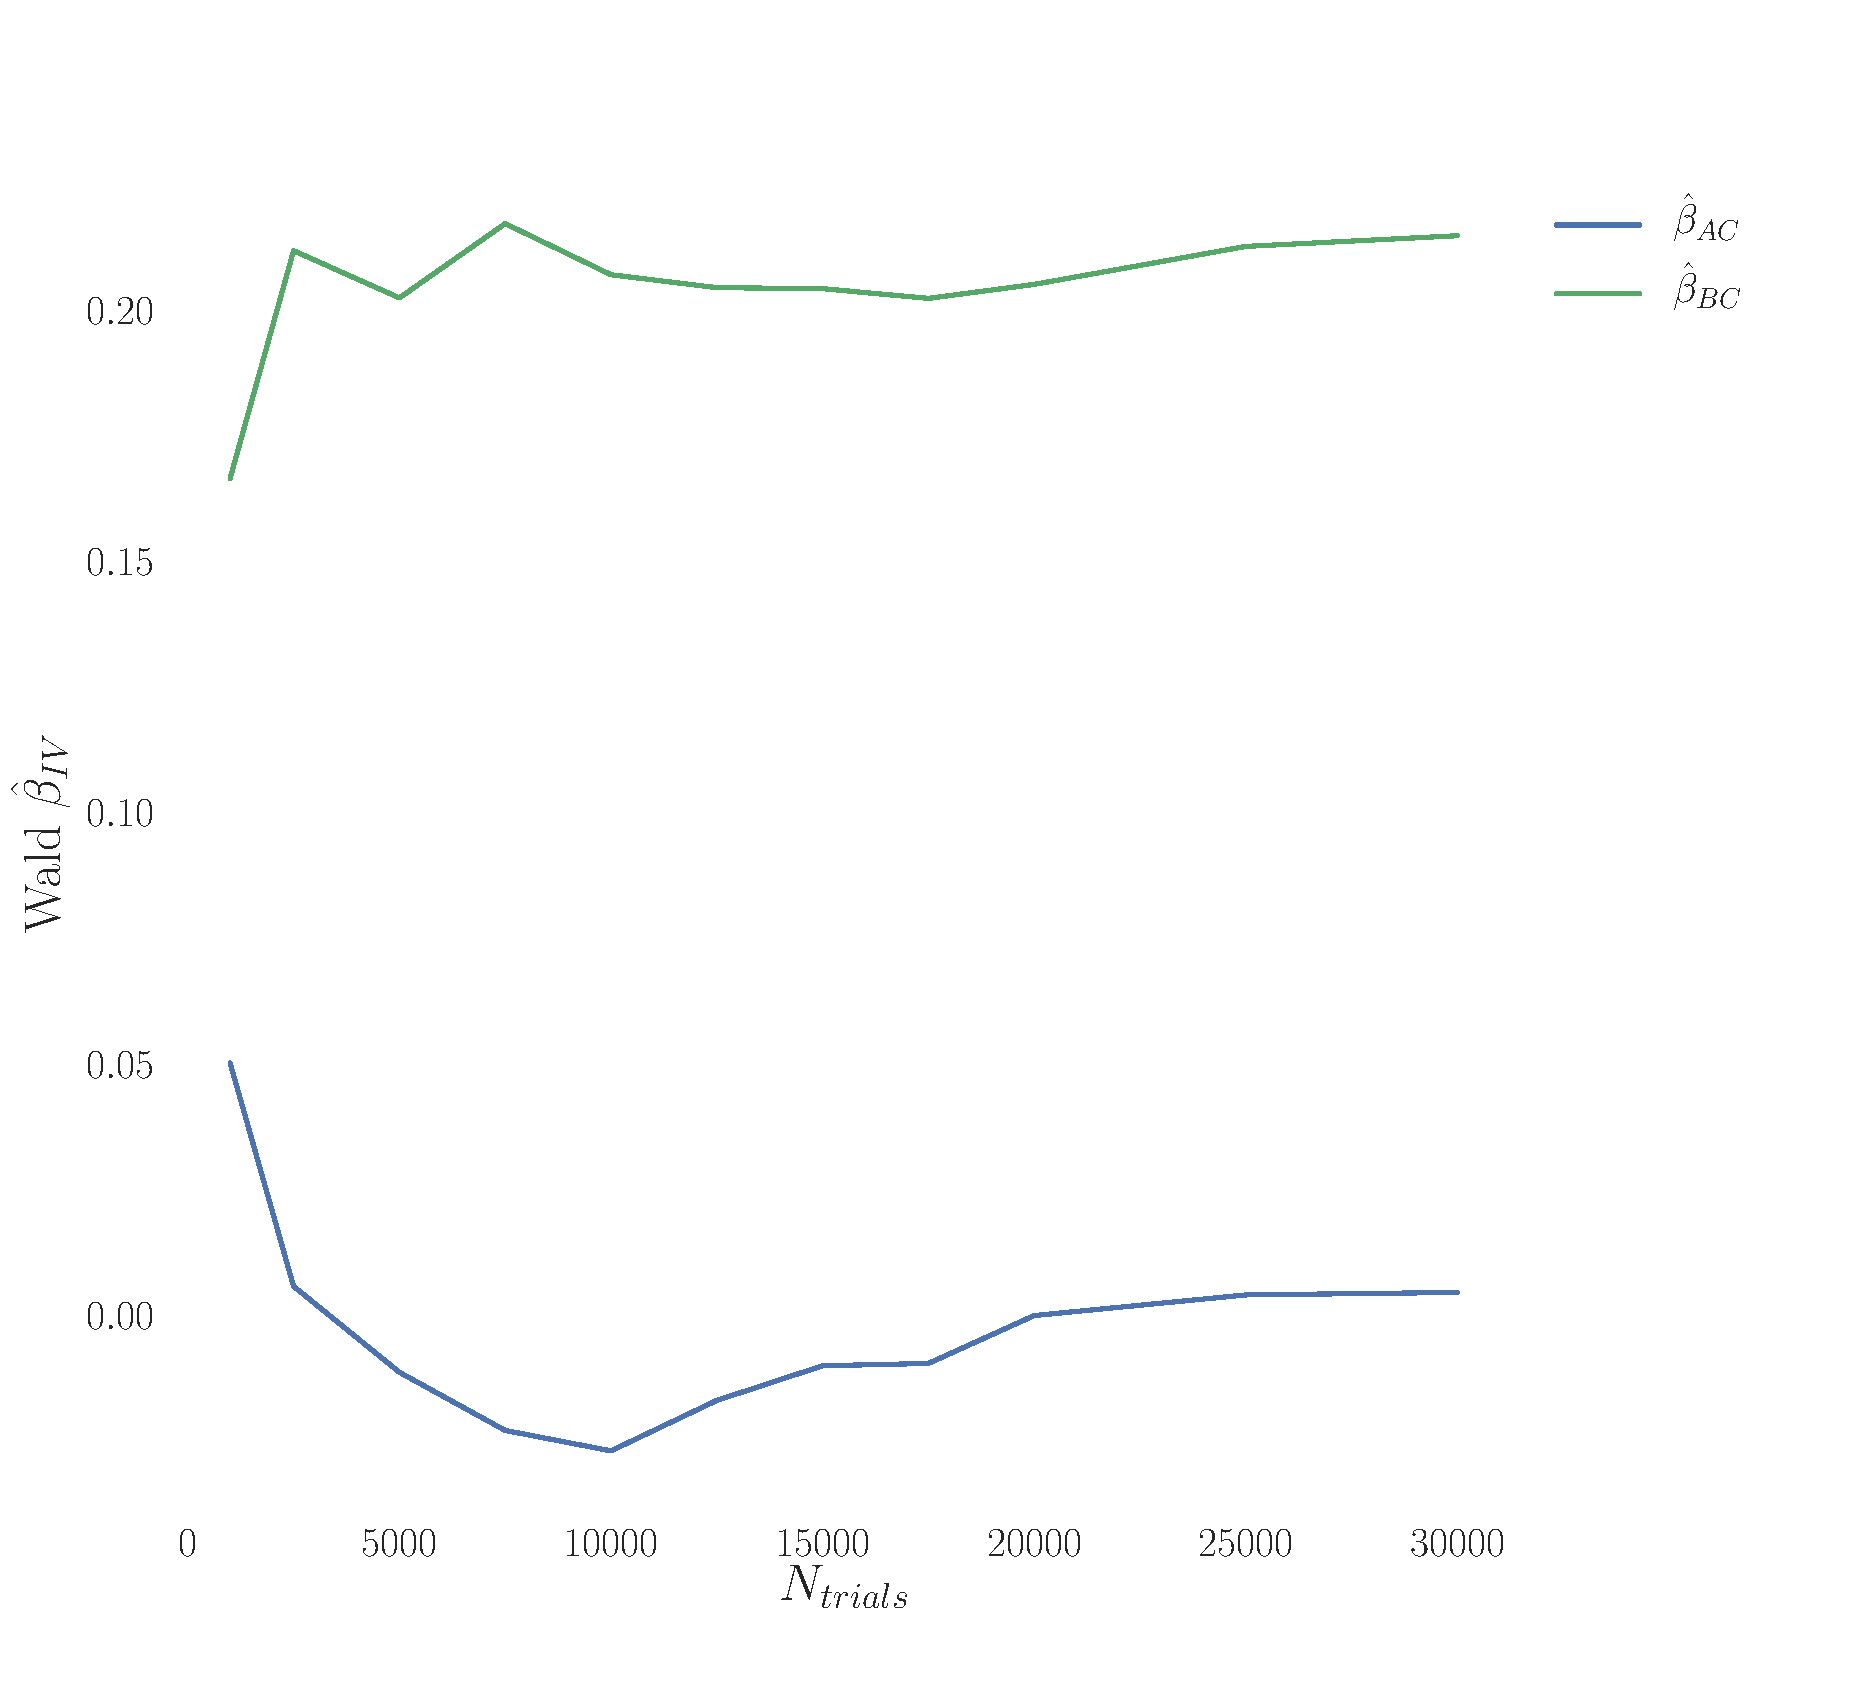
\includegraphics[scale=.2]{wald_network}
\caption{} \label{fig:network-power:2}
\end{subfigure}

\caption{Power analysis of IV estimator. \label{fig:network-power}}
\end{figure}

\begin{figure}
\begin{subfigure}{0.485\textwidth} 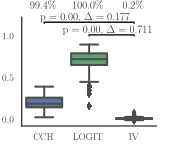
\includegraphics[scale=.25]{false_positive}
\caption{} \label{fig:network-class:1}
\end{subfigure}\hfill
\begin{subfigure}{0.485\textwidth} 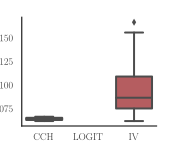
\includegraphics[scale=.25]{false_negative}
\caption{} \label{fig:network-class:2}
\end{subfigure}

\medskip
\begin{subfigure}{0.485\textwidth} 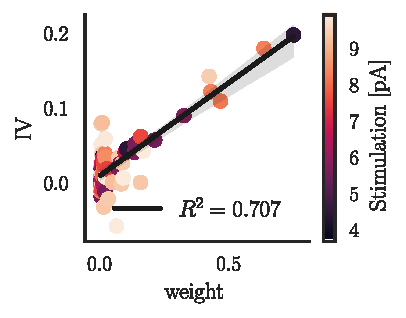
\includegraphics[scale=.25]{fit_wald}
\caption{} \label{fig:network-class:3}
\end{subfigure}\hfill
\begin{subfigure}{0.485\textwidth} 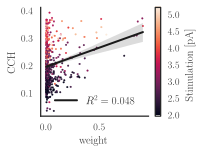
\includegraphics[scale=.25]{fit_cch}
\caption{} \label{fig:network-class:4}
\end{subfigure}
\caption{Comparing CCH and logit with IV \labelcref{fig:network-class:1,fig:network-class:2}. \label{fig:network-class}}
\end{figure}

\section{Discussion}
Spike time methods works well when network is desynchronized, small amplitude stimulation with close range. Our method opens up for the possibility of strong perturbations giving larger yield.
We are making the network results quite hard as all synapses have the same time constant such that multiple neurons are affecting the same cell at the same time for each stimulation

%Correlated refractory periods is *the* failure mode. How to randomize them

% Maybe nonlinearities in stimulation rescue old school approaches
Discuss distribution of V. Discuss 2p stimulation.  Conclude that there is absolutely no reason to hope things will work with 1p.

%Maybe some biophysics pecularity will rescue us
No way. But cite Buszaki.

%We recommend the WALD 
easily usable in the context of many experiment. Potentials for future improvement.

%brain regions versus neurons
IVs on multiple scales. 

%Causal inference techniques to fix experimental issues
Broad opportunity, cite RDD, cite diff-in-diff etc, broad overview of the promise of econometrics for neuro, matching

%Constructing good IVs
Multiple illuminations, designed sticky opsins


\FloatBarrier
\section{Methods}
\subsection{Instrumental variable estimation}
A simple approximation of the connectivity strength between putative sender and receiver neurons $ x $ and $ y $ respectively can be to ignore long distance excitation and simply calculate the relation between the spike times in $ x $ and $ y $ with a regression model given by

\begin{equation}
y = \beta x + u.
\label{eq:regress}
\end{equation}
Here $ y $ is the dependent variable, $ x $ is the explanatory variable, $ \beta $ is the slope of the $ x,y $ curve and $ u $ is an unknown error term. This system follows the causal path:
\begin{center}
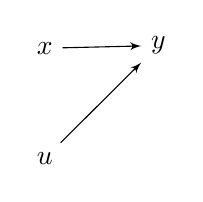
\begin{tikzpicture}
    \node (u) {$ u $};
    \node [above = of u] (x) {$ x $};
    \node [above right = of u] (y) {$ y $};
    \path [line] (x) -- (y);
    \path [line] (u) -- (y);
\end{tikzpicture}
\end{center}
Assuming that changes in spike times $ y $ are described by $ \beta x $ i.e. $ \de{y}{x} = \beta $ for spike times $ x $. One problem with this idea is that in a confounded system, perfectly correlated neurons will give statistically indistinguishable $ \beta $. In the extreme case where two neurons are both made to fire every time they are stimulated, they will have the same weights according to \cref{eq:regress}, after all, during stimulation  $ y=1 $ for both, even if only one of them drives the downstream neuron. Another problem is if the network state affects both the probability of a neuron to fire and also the probability of downstream neurons to fire. In this case, the network state can induce a correlation which will make the estimation highly biased. Arguably, the network state will, in all realistic models, have a dramatic influence on all neurons. In general, if multiple neurons are stimulated synchronously our estimates will be off, potentially massively so as seen in the equation
\begin{equation}
y = \beta x + u(x).
\end{equation}
Following the causal path

\begin{center}
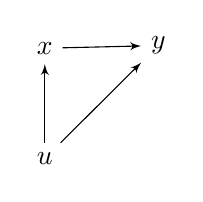
\begin{tikzpicture}
    \node (u) {$ u $};
    \node [above = of u] (x) {$ x $};
    \node [above right = of u] (y) {$ y $};
    \path [line] (x) -- (y);
    \path [line] (u) -- (x);
    \path [line] (u) -- (y);
\end{tikzpicture}
\end{center}
We now have the relation $ \de{y}{x} = \beta + \de{u}{x} $. To get at causality we thus require some stimulation that only highlight the activity in $ y $ caused by $ x $, however optogenetic stimulation is not specific enough as the photons will activate parts of the network activity $ u $. To have a remedy, we need something that can distinguish between different neurons that are stimulated. We thus require some instrument $ s_{r} $ which is (1) uncorrelated with the network $ u $ and (2) is correlated with the regressor $ x $\todo{cite the book or whatever}. The graph with stimulation is illustrated by

\begin{center}
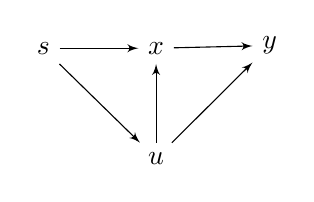
\begin{tikzpicture}
    \node (u) {$ u $};
    \node [above = of u] (x) {$ x $};
    \node [above right = of u] (y) {$ y $};
    \node [left = of x] (s) {$ s $};
    \path [line] (x) -- (y);
    \path [line] (u) -- (x);
    \path [line] (u) -- (y);
    \path [line] (s) -- (x);
    \path [line] (s) -- (u);
\end{tikzpicture}
\end{center}
The previous graph represents a confounded stimulation, however we may use the fact that a neuron that has fired just before the stimulation will be in absolute refractory period and hence have $ x_{s}=0 $. This introduces times where the spike from one of the stimulated neurons is missing. Neurons have low firing probability once we use small bins and are very noisy at spiking at small time scales. Thus if we assume that (1) the stimulation pattern is random (2) the network activity $ u $ is asynchronous and irregular we may use the refractory period as an instrumental variable illustrated in the following graph

\begin{center}
\begin{tikzpicture}
    \node (u) {$ u $};
    \node [above = of u] (x) {$ x $};
    \node [above right = of u] (y) {$ y $};
    \node [left = of x] (sr) {$ s_r $};
    \path [line] (x) -- (y);
    \path [line] (u) -- (x);
    \path [line] (u) -- (y);
    \path [line] (sr) -- (x);
\end{tikzpicture}
\end{center}
\todo[inline]{this will not work if you stimulate non random since then you may correlate u with sr, u is still driving x but asynchronously so sr is still uncorrelated with u.}
Here $ s_r $ represents times where the sender neuron is refractory during stimulation. This is then an estimator that compares the downstream activity when a given neuron is non-refractory with the downstream activity when it is, thus removing the confounding. The true $ \beta $ is given by
\begin{equation}
\beta_{IV} = \de{y}{s_r} / \de{x}{s_r}
\end{equation}
Since our instrument $ s_r $ is binary we may use the Wald estimator \todo{cite wald} to estimate $ \beta_{IV} $ by
\begin{equation}
 \hat{\beta}_{IV} = \frac{\bar{y}_{s} - \bar{y}_{s_r}}{\bar{x}_{s} - \bar{x}_{s_r}} = \bar{y}_{s} - \bar{y}_{s_r}
 \label{eq:wald}
\end{equation}
Here $ \bar{y}_s $ is the average number of trials where stimulating $ x $ resulted in a response in $ y $ and $ \bar{y}_{s_r} $ is the average number of trials where an unsuccessful stimulation resulted in a response in $ y $.

However the estimate of the refractory period $ s_r $ may be biased, as the network state may differ between times when a neuron is refractory and times when it is not. This issue we can also correct for by calculating $ \beta $ for baseline bins with no stimulation and no stimulation during absolute refractory period. This will linearly correct for the differences in network state that are due to refractory periods while maintaining the causal validity of \cref{eq:wald}.

\todo[inline]{Note that if we assume that the stimulation is so strong that the network effect $ u_{ns} $ has a negligible effect on $ x_{s} $ and that due to synaptic and axonal delay the effect of $ u_{s} $ is unable to affect $ x_{s} $ in it's respective stimulus response time. Then a conventional method like logistic regression will work.}

\subsection{Statistical testing on cross correlation histogram}
The statistical tests giving the probabilities $ p_{diff} $ and $ p_{fast} $ were done according to \cite{Stark2009, English2017}. Briefly, to test if the cross correlation histogram (CCH) peak was significant we employed two tests. By using the Poisson distribution with a continuity correction \cite{Stark2009} given by \cref{eq:poissoncontcor} we calculated $ p_{diff} $ by comparing the peak in positive time lag with the maximum peak in negative time lag \cite{English2017} and the difference from the CCH convoluted with a hollow Gaussian \cite{Stark2009}.
\begin{equation}
p(N|\lambda(m)) = 1 - \sum_{k=0}^{N-1}\frac{e^{-\lambda(m)}\lambda(m)^k}{k!} - \frac{e^{-\lambda(m)}\lambda(m)^N}{2N!}
\label{eq:poissoncontcor}
\end{equation}
Here $ \lambda $ represents the counts at bin $ m $ and $ N $ is the number of bins considered.
\subsection{Simulated network}
The first simple network consists of three leaky integrate and fire (LIF) neurons given in \cref{eq:LIF}:
\begin{equation}
	\tau \dot{V}_{i}(t) = -(V_{i}(t) - E_{L}) + RI_{i}(t).
    \label{eq:LIF}
\end{equation}
When the membrane potential $ V_{i} $ of neuron $ i $ reaches a threshold $ \theta $ an action potential is emitted and the depolarization is reset to the leak potential $ E_{L} $ followed by an absolute refractory period $ \tau_{rp} $. The membrane time constant is represented by $ \tau $ and $ I_{i}(t) $ denotes the synaptic currents arriving at the soma modeled as a sum of alpha functions given by
\begin{equation}
	\label{eq:syn}
	RI_{i}(t) = \sum_{j}J_{ij}\sum_{k}t\exp(-(t-t_{j}^{k})/\tau_{syn}) - D.
\end{equation}\todo{make sure delay is correctly inserted}
Different synapses are denoted by $ j = 1,...,C+C_{ext} $ with post synaptic potential (PSP) amplitude (synaptic efficacy) denoted as $ J_{ij} $. When neuron $ j $ emits it's $ k $'th spike at time $ t_{j}^k $ it arrives at neuron $ i $ at $ t = t_{j}^k + D $ where $ D $ denotes a transmission delay. Furthermore all neurons are driven by an external Poisson drive and an Gaussian noise process given in \cref{eq:channelgauss}.
\begin{equation}
	I(t) = mean + std * N_j for t_0 + j dt \leq t < t_0 + (j-1) dt 
    \label{eq:channelgauss}
\end{equation}
where $N_j$ are Gaussian random numbers with unit standard deviation and $t_0$ is 
the device onset time.
\todo[inline]{small perturbations on noisy networks will not yield a correlation between AC because the variance in stimulus response time in A will not be explained by the variance in spike times of C. Small variations of onset times in A relative to C will over many trials will wash out correlations between AC and at the same time strengthen correlations between BC. The only way to get a strong correlation between AC is to impose a short and strong stimulus effectively making AB spike coincidentally.}


%-------------------------------------------------------------------------------
%                                 REFS
%-------------------------------------------------------------------------------
\pagestyle{empty}
\bibliographystyle{apalike}
{\footnotesize\linespread{1}
\bibliography{library}}
%-------------------------------------------------------------------------------
%                                 TODOS
%-------------------------------------------------------------------------------
\newpage
\listoftodos
\end{document}
